\documentclass[11pt,letterpaper]{article}
\usepackage{naaclhlt2016}
\usepackage{times}
\usepackage{latexsym}
\usepackage{color}

% More packages
\usepackage{amsmath}
\usepackage{amssymb}
\usepackage{framed}
\usepackage{graphicx}
%\usepackage{hyperref}
\usepackage{xspace}

% Some helpful macros
%% Abbreviations
\newcommand{\encdec}{\textsc{EncDec}\xspace}
\newcommand{\attn}{\textsc{AttnBaseline}\xspace}
\newcommand{\attncopy}{\textsc{AttnCopy}\xspace}
\newcommand{\atis}{\textsc{ATIS}\xspace}
\newcommand{\regex}{\textsc{Regex}\xspace}
\newcommand{\geo}{\textsc{Geo}\xspace}

\newcommand{\catroot}{\textsc{Root}\xspace}
\newcommand{\catquotstr}{\textsc{Str}\xspace}
\newcommand{\catint}{\textsc{Int}\xspace}
\newcommand{\catstate}{\textsc{State}\xspace}
\newcommand{\catstateid}{\textsc{StateId}\xspace}

%% Mathematical Notation
\newcommand{\vocabin}{\mathcal{V}^{\text{(in)}}}
\newcommand{\phiin}{\phi^{\text{(in)}}}
\newcommand{\vocabout}{\mathcal{V}^{\text{(out)}}}
\newcommand{\phiout}{\phi^{\text{(out)}}}
%\newcommand{\vocabin}{\mathcal{V}}
%\newcommand{\phiin}{\phi}
%\newcommand{\vocabout}{\overline{\mathcal{V}}}
%\newcommand{\phiout}{\overline{\phi}}

%% Formatting
\newcommand\nl[1]{\textit{#1}}

% Other
\newcommand{\aster}{{\normalsize \textsuperscript{*}}\xspace}

%\naaclfinalcopy % Uncomment this line for the final submission
\def\naaclpaperid{***} %  Enter the naacl Paper ID here

% To expand the titlebox for more authors, uncomment
% below and set accordingly.
% \addtolength\titlebox{.5in}    

\newcommand\pl[1]{\textcolor{red}{[PL: #1]}}
\newcommand\rj[1]{\textcolor{blue}{[RJ: #1]}}

% Hide comments, see actual page count
\renewcommand\pl[1]{\iffalse #1 \fi}
\renewcommand\rj[1]{\iffalse #1 \fi}

\newcommand\BibTeX{B{\sc ib}\TeX}


%\title{Recurrent Neural Network Semantic Parsing with Compositional Data Augmentation}
% PL: less clunky
\title{Neural Semantic Parsing with Compositional Data Augmentation}
\author{Robin Jia\\
	    Computer Science Department\\
      Stanford University\\
	    {\tt robinjia@stanford.edu}
	  \And
    Percy Liang\\
    Computer Science Department\\
  	Stanford University\\
  {\tt pliang@cs.stanford.edu}}

\date{}

\begin{document}

\maketitle

\begin{abstract}
Building accurate semantic parsers currently requires substantial effort
with lexicons, grammars, and feature engineering.
This paper presents a much simpler approach to semantic parsing that uses
recurrent neural networks (RNNs).
%which has shown promise for many other NLP tasks.
Vanilla RNNs are insufficient to capture the crisp structural regularities of
semantic parsing,
so we propose two mechanisms to address this.
\rj{I like period instead of colon}
First, we introduce a new attention-based copying mechanism that
allows the parser to generalize to unseen entities.
Second, we introduce a new data augmentation scheme
that injects prior knowledge about compositionality into the parser.
Our system achieves good accuracy on three semantic parsing datasets.
%including new state-of-the-art numbers on the \regex domain.
\end{abstract}

\section{Introduction}
\begin{figure}[t] 
\small
\begin{center} 
  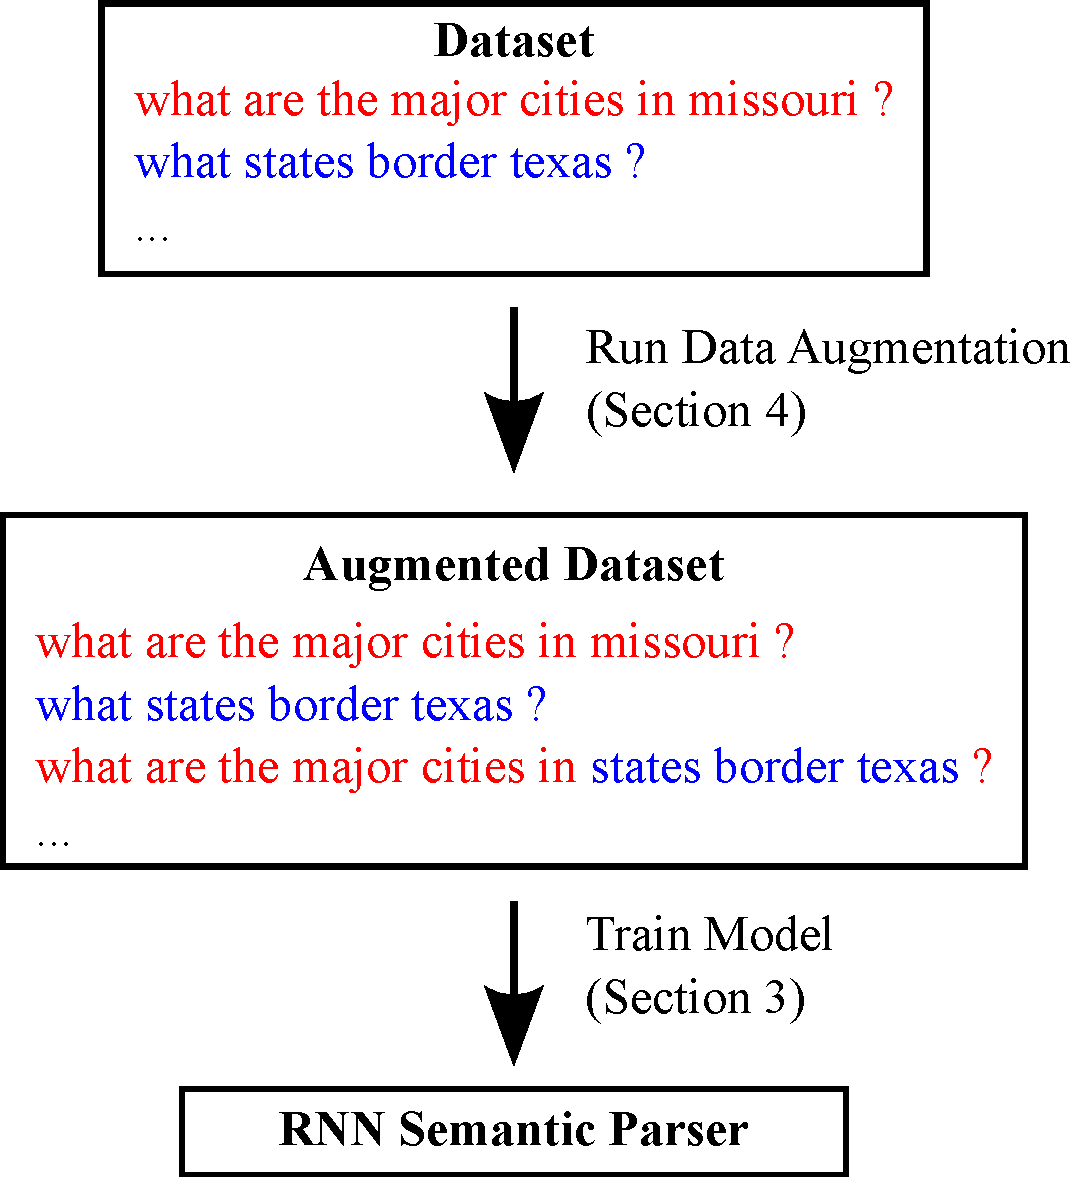
\includegraphics[scale=0.35]{fig-overview.pdf}
\end{center} 
\caption{An overview of our system.
  \rj{What do you think of this?  It's easier to do this figure
    if everything moves down vertically, and I think the colors
  make it clearer what's going on.
My biggest issue with this figure is that there's no picture of an RNN.}
}
\rj{Yea or nay on the square brackets?}
\label{fig:overview}
\end{figure}

% Semantic parsing is useful, but complicated
Semantic parsing---the precise translation of natural language utterances into 
logical forms---has many applications,
including question answering \cite{zelle96geoquery,zettlemoyer05ccg,zettlemoyer07relaxed,liang11dcs,berant2013freebase},
instruction following \cite{artzi2013weakly},
and regular expression generation \cite{kushman2013regex}.
Modern semantic parsers \cite{artzi2013uw,berant2013freebase} are complex pieces of software,
requiring not just hand-crafted features,
but also the definition of lexicons and grammars,
which is both important and fragile.
\rj{``which are''?  I'm not sure what is being called important and fragile}
%with a great deal of hand-crafted knowledge baked into their internal structure;
%Frameworks like CCG \citep{zettlemoyer05ccg} must deal with complex lambda calculus expressions,
%and systems like SEMPRE \cite{berant2013freebase}
%require large amounts of code that define the parser's grammar and features.
% TODO: argue this better

% Comment about our model being general-purpose, maybe delete
%Some recent work has tried to make semantic parsing
%into a general purpose technology \cite{wang2015overnight},
%but the accuracy of these systems leaves much to be desired.
%\pl{the main complaint should be about complexity, not accuracy,
%since in the end, we don't really gain on that}
%\rj{The idea of this sentence was to foreshadow improvements on overnight.
%I'll take it out if we wind up not running those experiments.}
%\pl{in general, use 'accuracy' rather than 'performance' since it's more precise;
%systems people use performance to talk about speed}

% RNNs are great!
Meanwhile, recurrent neural networks have made swift inroads into 
many structured prediction tasks in NLP,
including machine translation
\cite{sutskever2014sequence,bahdanau2014neural} and
syntactic parsing \cite{vinyals2015grammar,dyer2015transition},
achieving state-of-the-art results with minimal feature engineering.
So the natural question is, 
%can we leverage RNNs for semantic parsing?
can we use RNNs to build an accurate semantic parser?  % RJ: IMO this makes the transition to next paragraph easier

%computing convex hulls \cite{vinyals2015pointer}.
%RNNs are also appealing for their simplicity, as they require 
%little hand-engineering of features.
%Even though RNNs generate their output in a linear fashion,
%work on syntactic parsing has demonstrated that they can learn
%to generate linearized representations of tree-structured outputs as well
%\cite{vinyals2015grammar}.

% Datasets small, RNNs don't have built in compositionality
% PL: let's not emphasize that our datasets are small, but the modeling challenges
%The drawback of these RNN models is that they require
%large amounts of data to achieve good accuracy.
%\newcite{sutskever2014sequence} trained their
%neural machine translation model on 12 million sentences;
%\newcite{vinyals2015grammar} trained their
%neural syntactic parser on datasets of at least 40 thousand sentences,
%and used millions of sentences to achieve their best results.
%In contrast, semantic parsing datasets often consist of only 
%hundreds of labeled examples.

Two major challenges stand in the way.
First, semantic parsers must be able to generalize to 
a large set of entities that may not appear during training.
Second, semantic parsers must understand compositionality:
they must be able to recognize
hard alignments between fragments of utterances and logical forms,
and know about the predictable ways in which these fragments can be combined.
RNNs do not intrinsically have a concept of compositionality,
and can only learn about these crisp structural regularities
by observing data.

%\pl{be careful - I think we need to explain what we mean by 'compositionality'}
%\pl{in general, can tighten this paragraph;
%somehow the 'datasets are small, models are generic' message needs to come out more}
%\pl{I'd carve up the two problems as follows:
%  (i) handle unseen entities (need to explain this with concrete example, ideally in Figure 1);
%(ii) handle compositionality (need to explain this more, referencing example in Figure 1)}

% RNN model (handle unseen entities?), data augmentation (handle compositionality?)
In this paper, we present the first
semantic parser that uses a sequence-to-sequence RNN model to generate
logical forms.  
Our contributions are twofold.
First, we introduce an attention-based copying mechanism 
that allows our RNN model to generalize to unseen entities.
Second, to teach the model about compositionality,
we introduce compositional data augmentation,
which induces a high-precision grammar from the training data
and augments the training data with new examples sampled from this grammar.

%\pl{
%Overall good - flows well and well-motivated, generally like the writing style.
%Currently, you do a good job of giving background about RNNs
%and the challenges that arise when applying to semnatic parsing.
%But the main thing that you need to do more of is highlight our contributions
%and connect it directly with challenges.
%Make it really crisp - don't go for subtlety here: for example,
%say there are two challenges, A, and B.  We tackle A using C and B using D.
%Make our contributions sound as exciting as the challenges!
%}

\section{Task}
\begin{figure}[t] 
\small
\begin{framed}
\footnotesize
\subsubsection*{\geo}
\textbf{Input}: \nl{what is the population of iowa ?}\\
\textbf{Output}:

\quad \texttt{\_answer ( A , ( }

\qquad \texttt{\_population ( B , A ) ,}

\qquad \texttt{\_const ( B , \_stateid ( iowa ) ) ) )}

\subsubsection*{\regex}
\textbf{Input}: \nl{lines using ` abc ' after ` def '}\\
\textbf{Output}: \texttt{. \aster def . \aster abc . \aster}

\subsubsection*{\atis}
\textbf{Input}: \nl{can you list all flights from chicago to milwaukee}
\textbf{Output}:

\quad \texttt{( \_lambda \$0 e ( \_and ( \_flight \$0 )}

\qquad \texttt{( \_from \$0 chicago : \_ci )}

\qquad \texttt{( \_to \$0 milwaukee : \_ci ) ) )}
\end{framed}
\caption{One example from each of our three domains.}
\label{fig:task}
\end{figure}

We frame semantic parsing as a generic sequence-to-sequence task.
The input utterance $x$ is represented as a sequence of words $x_1, \dotsc, x_m
\in \vocabin$, the input vocabulary;
similarly, the output logical form $y$ is represented
as a sequence of tokens $y_1, \dotsc, y_n \in \vocabout$, the output vocabulary.
A linear sequence of tokens might appear to lose the hierarchical structure of a logical form,
%instead of an abstract syntax tree may seem unnatural,
%but this choice makes it easier to define our RNN model.
but there is precedent: \newcite{vinyals2015grammar}
showed that an RNN can reliably predict tree-structured outputs
in a linear fashion.
Figure~\ref{fig:task} shows sample input-output pairs for the different
datasets used in this paper.

\subsection{Datasets}
%\begin{table}[t]
%  \centering
%  \small
%  \begin{tabular}{|l|c|c|c|}
%    \hline
%    Dataset & Training Examples & Test Examples \\
%    \hline
%    \atis & 4473 & 448 \\
%    \regex & 660 & 164 \\
%    \geo & 600 & 280 \\
%    \hline
%  \end{tabular}
%  \caption{Overview of the datasets used in this paper.  
%  Note that For \regex, we create our own split by randomly partitioning the dataset.}
%  \label{tab:datasets}
%\end{table}

We evaluate our system on three standard semantic parsing datasets:
\begin{itemize}
  \item \textbf{GeoQuery} (\geo) contains
  natural language questions about US geography
  paired with corresponding database queries.
  We use the standard split of 600 training examples and 280 test examples
  introduced by \newcite{zettlemoyer05ccg}.

  \item \textbf{Regular Expressions} (\regex)
  contains natural language descriptions of regular expressions
  paired with associated regular expressions.
  Unlike \newcite{kushman2013regex}, 
  we evaluate on a test set of $164$ examples selected randomly
  from the dataset.
%  however, to compare with their results, we also evaluate
%  with 3-fold cross-validation.

  \item \textbf{ATIS} (\atis) contains 
    natural language queries for a flights database
    paired with corresponding database.
    We train on $4473$ examples and evaluate on the $448$
    test examples used by 
    \newcite{zettlemoyer07relaxed}.
\end{itemize}

%It is notable that these datasets are many orders of magnitude smaller
%than those used to train neural machine translation systems
%\cite{sutskever2014sequence,bahdanau2014neural}.

In this work, we only explore learning from logical forms.
We therefore do not use any semantic parsing datasets
that only include denotations,
such as \textsc{WebQuestions} \cite{berant2013freebase}.

%\pl{no intrinsic reason why we can't have denotations;
%state in a more neutral way}

\section{RNN Model}
\begin{figure}[t] 
\small
\begin{center} 
  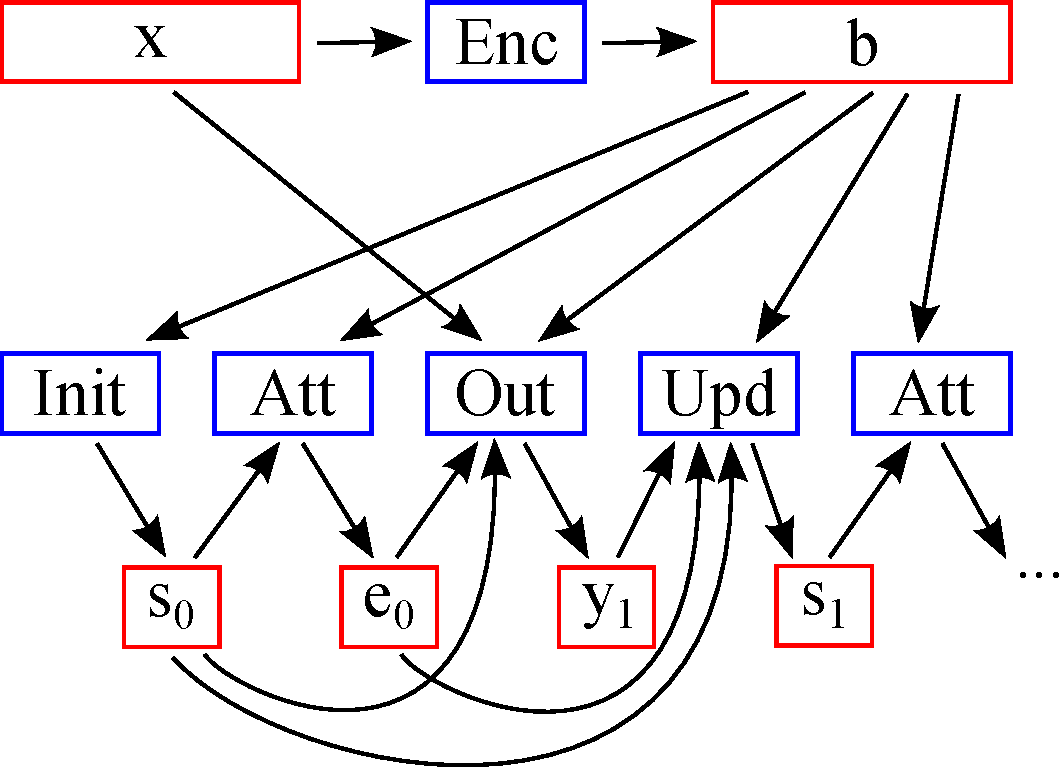
\includegraphics[scale=0.4]{fig-rnn.pdf}
\end{center} 
\caption{An overview of our RNN model.  
  Enc, Encoder; Init, Decoder Initialization;
  Att, Decoder Attention; Out, Decoder Output;
  Upd, Decoder Update.
}
\label{fig:rnn}
\end{figure}
Our neural semantic parser is backed by a generic sequence-to-sequence RNN model.
This model is based closely on existing 
attention-based neural machine translation models
\cite{bahdanau2014neural,luong2015translation},
but also includes a novel attention-based copying mechanism.

\pl{we should have a paragraph after our description
  or in discussion comparing our model with neural MT models;
  doing a careful diff is important }
  \rj{It's basically the same as Thang's other than the output module}

At a high level, our system consists of two main modules:
\begin{enumerate}
  \item \textbf{Encoder Module}.  This module 
    converts the input sequence $x_1, \dotsc, x_m$
    into a sequence of \emph{context-sensitive embeddings}
    $b_1, \dotsc, b_m$,
    where each $b_i$ is a real-valued fixed-dimensional vector.
  \item \textbf{Decoder Module}.  This module
    takes in the input sequence and context-sensitive embeddings,
    and generates a probability distribution
    over sequences $y = y_1, \dotsc, y_n$,
    where each $y_j \in \vocabout$.
    It writes the output tokens one at a time,
    maintaining a hidden state $s_j$ at each time $j$.
    It generates the next output token $y_{j+1}$ based on $s_j$,
    then updates the hidden state to $s_{j+1}$ based on
    $s_j$ and $y_{j+1}$
\end{enumerate}
The decoder itself can be decomposed into four modules:
\begin{enumerate}
  \item \textbf{Initialization Module}:
    Takes in the context-sensitive embeddings $b_1, \dotsc, b_m$, and
    outputs the initial decoder hidden state $s_0$.
  \item \textbf{Attention Module}:
    Takes in $b_1, \dotsc, b_m$ and the current state $s_j$,
    and outputs an attention score vector $e_j$ of length $m$.
  \item \textbf{Output Module}.  
    Takes in $b_1, \dotsc, b_m$, $s_j$, $e_j$, and $x$,
    and outputs a probability distribution 
    for $y_{j+1}$, the next word to write.
  \item \textbf{Update Module}: 
    Takes in $b_1, \dotsc, b_m$, $s_j$, $e_j$, and $y_{j+1}$,
    and outputs the new state $s_{j+1}$.
\end{enumerate}
\pl{Move the second sentences in the three bullets into 'Decoder Module'
  and cut the first sentence.
  This text is currently taking up a lot of space and kind of wordy.
}
\rj{I couldn't really see moving it all into "Decoder Module".  How does this look?
Also, I realized that 4 modules makes more sense than 3.}
Figure~\ref{fig:rnn} illustrates how these modules are connected
to form the overall RNN model.
In the next sections, we describe these modules in greater detail.

%\pl{
%Think about good software engineering principles when you're defining the
%model.  What I mean is start by the abstract interfaces
%with modules Encode, Decode, etc.
%Define their types (sequence to vector, distribution over tokens, etc.)
%and give intuition about what they are supposed to do;
%forward reference the sections that talk about the modules.
%Absolutely don't just start jumping into model details.
%Start top-down.
%}

\pl{
  Also need at least one (probably two) figure(s)
  to illustrate (i) the abstract model framework,
  and (ii) a concrete example.  Use the same example as in Figure 1.
}
\rj{First figure made.  Second figure seems like it would need to be quite big?}


\subsection{Encoder Module}
The encoder is a bidirectional RNN \cite{bahdanau2014neural}.
First, a word embedding function $\phiin$ 
maps each word $x_i$ to a fixed-dimensional vector.
These vectors are fed as input to two RNNs: a forward RNN and a backward RNN.
The forward RNN starts with an initial hidden state $h_0^{\text{F}}$,
and generates a sequence of hidden states $h_1^{\text{F}}, \dotsc, h_m^{\text{F}}$ by
repeatedly applying the recurrence 
\begin{align}
  h_i^{\text{F}} = \text{LSTM}(\phiin(x_i), h_{i-1}^{\text{F}}).
\end{align}
The recurrence takes the form of an LSTM \cite{hochreiter1997lstm}.
\pl{technically, does $h_i$ need to include the cell variables?}
\rj{In this case, yes. I didn't try excluding the cell.}
\pl{technically, LSTM refers to the entire model, not just one local update}
\rj{I've seen this phrasing elsewhere
e.g. http://arxiv.org/pdf/1409.0473v6.pdf bottom of page 2.
Do you think saying ``LSTM unit'' is better?}
The backward RNN similarly generates hidden states $h_m^{\text{B}}, \dotsc, h_1^{\text{B}}$
by processing the input sequence in reverse order.
Finally, we define 
the context-sensitive embedding
$b_i$ to be the concatenation of $h_i^{\text{F}}$ and $h_i^{\text{B}}$.
\pl{$\phiin(x_i)$ is notationally pretty clunky; come up with a single letter?}
\pl{what's $\phi(x_i)$?}
\rj{is this better?}

\subsection{Decoder Initialization Module}
Let $h$ be the concatenation of $h_m^{\text{F}}$ and $h_1^{\text{B}}$.
The decoder's initial state $s_0$ is
\begin{align}
  s_0 = \tanh(W^{(i)} h),
\end{align}
where $W^{(i)}$ is a parameter matrix.

\subsection{Decoder Attention Module}
At each time step $j$, and for each word $x_i$ in the input,
we compute an attention score $e_{ji}$.
We use the general content-based scoring function of
\newcite{luong2015translation}:
\begin{align}
  e_{ji} = s_j^\top W^{(a)} b_i,
\end{align}
where $W^{(a)}$ is a parameter matrix.

\subsection{Decoder Update Module}
Our decoder update step is the same as \newcite{bahdanau2014neural}.
At each time step $j$, the scores $e_j$ 
from the attention module are converted to a probability distribution 
over $\{1, \dotsc, m\}$ with a softmax:
\begin{align}
  \alpha_{ji} = \frac{\exp(e_{ji})}{\sum_{i=1}^m \exp(e_{ji})}.
\end{align}
$\alpha_{ji}$ is known as the attention weight \cite{bahdanau2014neural},
and can be interpreted as the amount of attention
paid to the $i$-th input word at time step $j$.
Then, a context vector $c_j$ is computed as a weighted average of the $b_i$'s:
\begin{align}
  c_j = \sum_{i=1}^m \alpha_{ji} b_i.
\end{align}
The current input vector $v_{j+1}$ is computed as 
the concatenation of $\phiout(y_{j+1})$ and $c_{j}$,
where $\phiout$ is another word embedding function.
Finally, the state is updated according to the recurrence
\begin{align}
  s_{j+1} = \text{LSTM}(v_{j+1}, s_j).
\end{align}

\subsection{Decoder Output Module}
Finally, we describe two decoder output modules: a baseline module, and a
more sophisticated module that performs attention-based copying.

\subsubsection{Baseline}
\label{sec:baseline-output}
The baseline output module uses a simple softmax over all
output vocabulary words.
At each time step $j$, it first computes the context vector $c_j$ ,
as in the update module.
Given $c_j$ and $s_j$, the probability of outputting word $w \in \vocabout$ 
as the next word $y_{j+1}$ is
\begin{align}
  P(y_{j+1} = w \mid x, y_{1:j}) \propto \exp(M_{w} s_j + U_w c_j),
\end{align}
where $M$ and $U$ are matrices with rows indexed by elements of $\vocabout$.

\subsubsection{Attention-based Copying}
One of the main contributions of this paper is a 
novel attention-based copying mechanism,
which improves upon the baseline output module.
This new mechanism is motivated by the need 
to generalize well to a large set of entity names,
including ones that were not seen at training time.
Often times, these entity names
can be copied directly from the input to the output.
For example, in Figure~\ref{fig:task},
the word ``iowa'' could be copied from the input
to the output.
Similarly, other place names in \geo and \atis can be copied,
as well as quoted strings in \regex.

Our proposed attention-based copying mechanism
enables the network to copy a word directly from input to output,
with probability determined by the amount of attention paid to that input word.
Formally, we have
\begin{align}
  P(&y_{j+1} = w \mid x, y_{1:j}) \propto 
  \\ & \exp(M_{w} s_j + U_w c_j)
  + \sum_{i=1}^m \mathbb{I}[x_i = w] \exp(e_{ji}).
\end{align}
We note that our attention-based copying can be seen as a 
combination of a standard softmax output layer
and a Pointer Network \cite{vinyals2015pointer}.  In a Pointer Network,
the only way to generate output is to copy a symbol from the input
using an attention mechanism.

\subsection{All Models}
We define a total of three models (one main model and two baselines):
\begin{itemize}
  \item \textbf{\attncopy}.  This is our full model with attention-based copying.
  \item \textbf{\attn}.  The is same as \attncopy, except with the baseline 
    output module.
  \item \textbf{\encdec}.  This baseline is an encoder-decoder model 
    \cite{sutskever2014sequence}
    that uses the baseline decoder output module.  
    This can be thought of as a variant of the \attn model
    where the Decoder Initialization module
    just returns $s_0 = h_m^{\text{F}}$,
    and the context vector $c_j$ is artificially set to always be $0$.
\end{itemize}

\subsection{Learning}
During training, we maximize log-likelihood of the annotated logical form.
We train the model using stochastic gradient descent.
Gradients are computed automatically using Theano \cite{bergstra2010theano}.

\section{Compositional Data Augmentation}
The strength of deep learning models lies in their flexibility.
However, this flexibility also presents a challenge:
because neural models make fewer assumptions about the task,
they can be at a disadvantage compared to specialized systems
that have domain knowledge baked in.

Our solution to this problem is to
augment our training datasets with new examples
generated from the original training examples.
This approach allows us to inject prior knowledge into our system,
as the new examples can be generated 
in a way that leverages domain knowledge.

For semantic parsing, one important phenomenon to model is compositionality.
There are often hard alignments between fragments
of the input and output, and these units can be composed
with each other in predictable ways.
We therefore propose a \emph{compositional data augmentation} scheme
that uses an induced grammar to generate new, highly structured examples.
We focus primarily on applying this to the \geo domain.
More details are shown in Figure~\ref{fig:augment-geo}.

\begin{figure}[t] 
\small
\begin{framed}
\footnotesize
\subsubsection*{Induced Rules}
Example 1: \nl{what states border illinois ?}\\
Induced rules:

\quad \catroot $\to$ \nl{what states border \catstate { }?}

\quad \catstate $\to$ \nl{states border \catstateid}

\quad \catstateid $\to$ \nl{illinois}

Example 2: \nl{what is the highest mountain in colorado ?}\\
Induced rules:

\quad \catroot $\to$ \nl{what is the highest mountain in \catstate { }?}

\quad \catstateid $\to$ \nl{colorado}

\subsubsection*{New Examples} 
\nl{what states border states border illinois?} \\
\nl{what states border states border colorado?} \\
\nl{what is the highest mountain in states border illinois?} \\
\nl{what is the highest mountain in states border colorado?}
\end{framed}
\caption{Data augmentation on \geo.  Due to lack of space,
we only show the grammar over utterances.
Analogous non-terminals and rules also exist for cities and rivers.}
\label{fig:augment-geo}
\end{figure}

This procedure begins by identifying \emph{high-precision alignments}
between pieces of an utterance and associated logical form.
First, for each $(x, y)$ pair, there is a trivial alignment that
matches the entire utterance with the entire logical form
(e.g. \nl{what states border illinois ?} aligns to an entire logical form).
We write some manual rules to convert questions into noun phrases
by stripping things like question marks and ``wh'' words
(e.g. to create \nl{states border illinois}).
Finally, we match entity mentions in the 
input and output based on simple string matching (e.g. \nl{illinois}).

These high-precision alignments allow us to
induce a simple grammar over pairs of utterances and logical forms.
This grammar can replace individual entity mentions with
other entities of the same type,
or with entire phrases that evaluate to a set of entities of the same type.
We then generate new examples from this grammar,
and add these to our original training dataset.

Our augmentation scheme is notable in that it 
transforms both the inputs and outputs simultaneously.
In contrast, other data augmentation techniques used in computer vision
\cite{krizhevsky2012imagenet}
only transform inputs without changing any output labels.

Our procedure generates examples that are on average
longer than the examples in the training and test sets.
Later, we explore in greater detail the ramifications of augmenting the training dataset
with examples drawn from a distribution that is very different from the test distribution.
\rj{Need to point this out first here, but leave main discussion to experiments section}

\subsection{Augmentation on \regex}
%\begin{figure}[t] 
%\small
%\begin{framed}
%\footnotesize
%\subsubsection*{Basic Rules}
%\catint $\to ($``0''$, 0) \mid ($``1''$, 1) \mid \dotsb \mid ($``9''$, 9)$
%
%\pl{something for quoted string?}
%\rj{No, those are all created from the training data}
%
%\subsubsection*{Induced Rules}
%Example: (``lines starting with `abc' '', \texttt{"abc.*"})\\
%Induced rules:
%
%\quad \catroot $\to$ (``lines starting with ` \catquotstr ' '', \texttt{"}\catquotstr\texttt{.*"})
%
%\quad \catquotstr $\to$ (``abc'', \texttt{"abc"}) \\
%
%Example: 
%
%\quad (``lines using more than 4 characters'', \texttt{".*.\{5,\}.*"})\\
%Induced rules:
%
%\quad \catroot $\to$ (``lines using more than \catint characters'', 
%
%\qquad \qquad \qquad \texttt{".*.\{(\catint + 1),\}.*"})
%
%\subsubsection*{Generated Examples} 
%(``lines starting with `hi' '', \texttt{"hi.*"})
%
%(``lines using more than 6 characters'', \texttt{".*.\{7,\}.*"})
%
%\dots
%\end{framed}
%\caption{Data augmentation on \regex.}
%\label{fig:augment-regex}
%\end{figure}
\regex and \atis have less nesting structure,
making them less suited for the compositional data augmentation scheme
described above.
However, we can still use high-precision alignment rules
to perform a simpler form of data augmentation.
We do this on \regex by looking for quoted strings and integers.
We generate new examples by
swapping quoted strings and integers in one example
for other quoted strings or integers.
%See Figure \ref{fig:augment-regex} for more detail.
%Similarly, on \atis, we identify city, airport, and airline,
%mentions using a lexicon extracted from the relational database
%that accompanies the \atis dataset,
%and replace entities in one example with a different entity
%of the same type.

Note that unlike our synthesized examples for \geo, 
these synthesized examples
are more like additional (non-independent) samples from the probability distribution
that generated the training data.

%The \atis domain presents a different set of challenges than
%\geo and \regex.  In particular, \atis boasts a larger number of
%entity types, as well as many entities that cannot be easily copied
%(e.g. airport names mapping to airport codes).
%
%To address these difficulties, we try a different data augmentation
%strategy for \atis, which we call lexicon-based data augmentation.
%From the relational database that accompanies the \atis dataset,
%we extract a lexicon mapping entity names to entity identifiers,
%for many of the most common entity types.
%We then add these pairs directly to the training dataset as new
%examples.
%\pl{wait, (dallas, dallas:ci) is an standalone example?
%there's no combination of examples?
%}
%\rj{Yes.} 
%\rj{I tried this because it was something we mentioned a while ago,
%  and it turned out this did better than the other augmentation strategies I tried.  
%But yeah, it's not very satisfying}

\section{Experiments}
We evaluate our system on three domains: \atis, \regex, and \geo.
For the \atis domain, we report exact logical form match accuracy.
For \regex, we determine correctness of a regular expression
by converting to deterministic finite automata (DFAs)
and checking equivalence, following \newcite{kushman2013regex}.
For \geo, we determine correctness based on denotation match.

\subsection{Implementation Details}
We tokenize logical forms in a domain-specific manner,
based on the syntax of the formal language being used.
We ensure that entity names can be easily copied from input to output.
At the same time, we perform name mangling on predicate names,
so that the model cannot cheat by copying these as well.
For example, in the \geo domain, we transform the name
of the predicate ``\texttt{state}'' to ``\texttt{\_state}.''
See Figure~\ref{fig:task} for examples.

We run all experiments with a hidden size of $400$ units.
Word vector sizes were chosen individually for each domain:
we used $50$ for \regex, $100$ for \geo, and $200$ for \atis.
We initialized all parameters uniformly at random 
within the interval $[-0.1, 0.1]$.
We used a simple learning rate schedule:
we first train the model for $25$ epochs at a learning rate of $0.1$,
then for $5$ more epochs with a learning rate of $0.05$,
and finally $5$ additional epochs with a learning rate of $0.025$.
We replace word vectors for words that occur only once in the training set 
with a universal \texttt{<unk>} word vector.

Another important hyperparameter is the number of
new examples to generate when performing data augmentation
For \geo, we train on the original dataset,
plus $300$ randomly sampled new examples.
For \regex, we train on the original dataset,
plus $200$ examples generated by swapping integers
and $200$ examples generated by swapping quoted strings.
%All hyperparameters were tuned by training on a subset of the
%training set, and evaluating on the remaining examples.

At test time, we use beam search with beam size $K=10$.
We automatically balance missing right parentheses
by adding them at the end.
We then pick the highest-scoring logical form that is valid.
On \geo, this means we take the highest-scoring parse
that does not yield an executor error when the
corresponding denotation is computed;
on \regex, this means that no error is thrown when 
converting the regular expression to a DFA.
On \atis, we always just pick the top prediction on the beam.

\subsection{Main Results}
\begin{table}[t]
  \centering
  \footnotesize
  \begin{tabular}{|l|c|c|c|}
    \hline
    & \atis & \regex & \geo \\
    \hline
    \textbf{Previous Work} & & & \\
    \newcite{zettlemoyer07relaxed} & $84.6$ & & \\
    \newcite{kushman2013regex} & & $65.5$ & \\
    \newcite{kwiatkowski10ccg} & & & $88.9$ \\
    \newcite{liang11dcs} & & & $91.1$ \\
    \hline
    \textbf{Original Dataset} & & & \\
    \encdec & $33.0$ & $7.3$ & $25.7$ \\
    \attn & - & $17.7$ & $76.4$ \\
    \attncopy & $74.3$ & $68.9$ & $85.7$ \\
    \hline
    \textbf{With Data Augmentation} & & & \\
    \encdec & & $7.9$ & $23.2$ \\
    \attn & & $17.7$ & $77.1$ \\
    \attncopy & & $68.9$ & $87.9$ \\
    \hline
  \end{tabular}
  \caption{Test accuracy on different datasets.}
  \rj{Note to self: ATIS + attncopy number is with a random initialization, not seeded}
  \label{tab:results}
\end{table}
We compare our system to state-of-the-art results
achieved on all three datasets (first group of rows of Table \ref{tab:results}).
On \geo, we list both \newcite{liang11dcs}
and \newcite{kwiatkowski10ccg}.
The former system achieved higher accuracy,
but it used a seed lexicon mapping words to predicates.
We explicitly avoid including such prior knowledge in our system.

First, we evaluate our system trained on the original dataset alone,
with no data augmentation.
Our results are summarized in the second section of Table \ref{tab:results}.
Note that we are roughly competitive with the state-of-the-art on \regex, 
although the numbers are not directly
comparable as the other work evaluates on different data.
However, we lag behind on \geo and \atis.

Training on the augmented datasets produces results shown in the
third section of Table~\ref{tab:results}.
We see that our compositional data augmentation improves 
our accuracy on \geo by more than two percentage points.
In contrast, we do not see accuracy gains on \regex, 
where we performed a less compositional form of data augmentation.

% RJ: Omitting this section for now.  The pictures don't look _that_ convincing
% I settled on using a large hidden state, which I think makes it
% less necessary to attend to exactly the right place.
% In particular, you see many instances where the network chooses to attend to the word
% after you would expect it to attend to.
% \subsection{Learning Compositionality via Alignments}

\subsection{Effect of Data Augmentation}
\begin{figure}[t] 
\small
\begin{center} 
  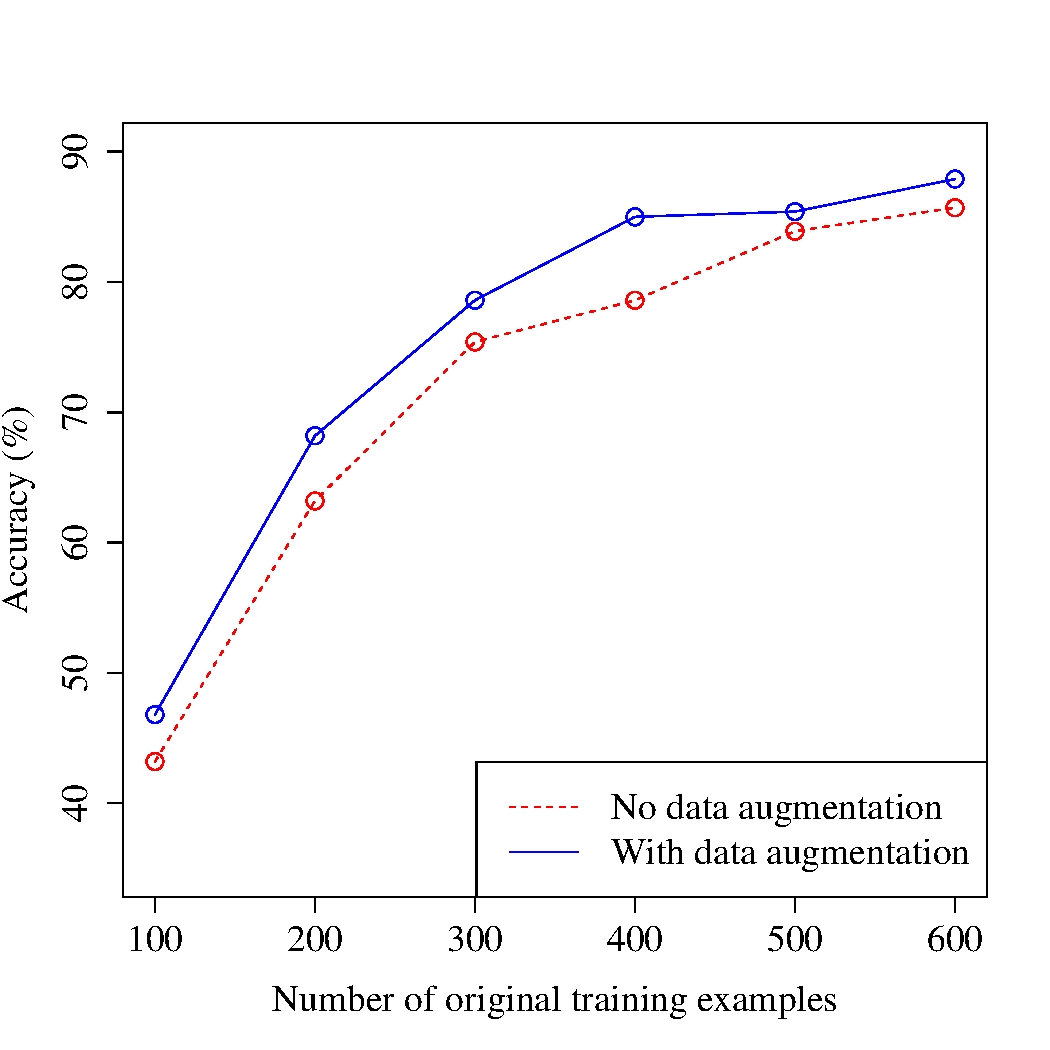
\includegraphics[scale=0.4]{fig-geo-augment.pdf}
\end{center} 
\caption{Accuracy on \geo as a function of number of training examples.
  Data augmentation gives a consistent accuracy boost,
regardless of original dataset size.}
\label{fig:geo-augment}
\end{figure}
\rj{Rewrote quite a bit here, as I think we maybe shouldn't
  focus so much on directly comparing the value of
real and synthesized examples, at least in this subsection}

To further measure the effects of compositional data augmentation,
we trained our system both with and without data augmentation
on various random subsets of the \geo dataset.
In Figure~\ref{fig:geo-augment}, we plot test accuracy as a function of
the number of real training examples.
As a heuristic, when doing data augmentation on $n$ real examples,
we always generate $\frac{n}2$ new examples.

From this plot, we see that data augmentation consistently boosts accuracy
across all dataset sizes.
In some cases, the synthesized examples prove to be
almost as helpful as real examples:
for example, training on $400$ real and $200$ synthesized examples
gets nearly the same accuracy as training on the full set of $600$ examples.

\subsection{Out-of-Domain Augmentation}
\begin{figure}[t] 
\small
\begin{framed}
\footnotesize
\subsubsection*{Depth-2 (same-domain)}

\textbf{Input}: \nl{rel:12 of rel:17 of ent:14}

\textbf{Output}: \texttt{( \_rel:12 ( \_rel:17 \_ent:14 ) )}

\subsubsection*{Depth-4 (out-of-domain)}

\textbf{Input}: \nl{rel:23 of rel:36 of rel:38 of rel:10 of ent:05}

\textbf{Output}: \texttt{( \_rel:23 ( \_rel:36 ( \_rel:38}

\qquad \qquad \quad \texttt{( \_rel:10 \_ent:05 ) ) ) )}

\end{framed}
\caption{A sample of our artificial data.}
\label{fig:artificial-data}
\end{figure}

\begin{figure}[t] 
\small
\begin{center} 
  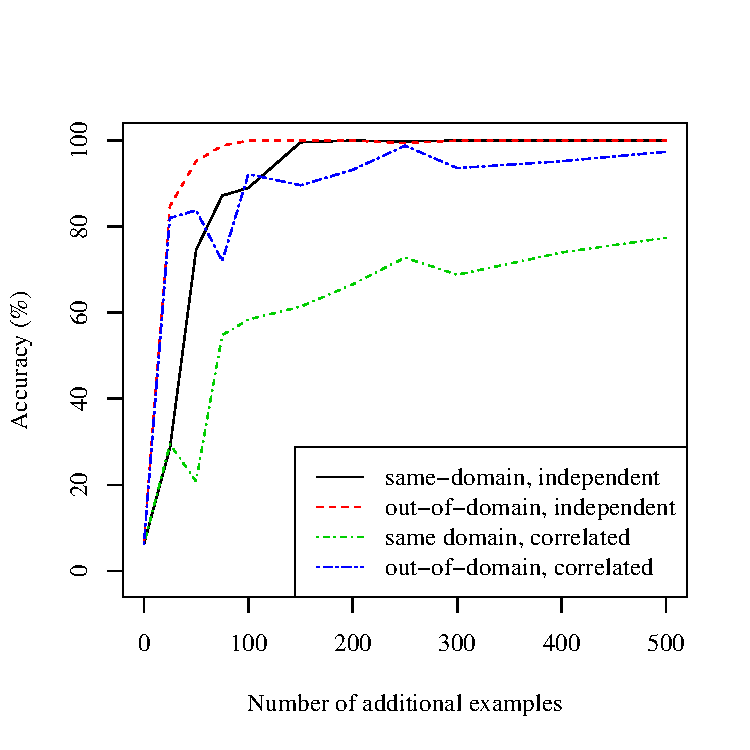
\includegraphics[scale=0.65]{fig-artificial-aug.pdf}
\end{center} 
\caption{Comparing augmentation methods on artificial data.}
\label{fig:artificial}
\end{figure}
% TODO: update this figure for the new experiments

%\begin{table}[t]
%  \centering
%  \small
%  \begin{tabular}{|l|c|}
%    \hline
%    Training Data & Accuracy (on Nested) \\
%    \hline
%    100 Nested (baseline) & $20.2\%$ \\
%    100 Nested + 100 Simple & $91.4\%$ \\
%    100 Nested + 100 Union & $95.0\%$ \\
%    200 Nested & $97.2\%$ \\
%    \hline
%  \end{tabular}
%  \caption{Results of the experiments on artificial data.}
%  \label{tab:artificial}
%\end{table}
Compositional data augmentation on \geo helped accuracy
even though the generated examples were not guaranteed
to be in the support of the test distribution;
meanwhile, data augmentation on \regex 
proved ineffective, even though 
the generated examples were similar to the test examples. 
One possible explanation is that by generating longer examples on
\geo, we biased the model to focus on examples that are similar to the
harder examples in the test set.
However, an interesting alternative explanation is that
data augmentation can in fact be most beneficial when the examples generated
do not match the test distribution.

More specifically, we wish to test two hypotheses.
First, we hypothesize that i.i.d. examples drawn from the test distribution 
may not help the model as much as i.i.d. examples
that are longer than those in the test distribution.
Second, we hypothesize that 
a similar claim holds when performing data augmentation,
which generates examples that are correlated with the initial training set.
Intuitively, longer examples could be helpful 
simply because they carry more information content per example,
or because their length forces the network to learn better alignments between
input and output tokens.

To investigate the effects of such \emph{out-of-domain} examples,
we conducted additional experiments on artificial data.
We constructed a simple world containing a set of entities
and a set of binary relations.
For any $n$, we can generate a set of depth-$n$ examples,
which involve the composition of $n$ relations
applied to a single entity.
Example data points are shown in Figure~\ref{fig:artificial-data}.
We train our model on various datasets,
then test it on a set of $500$ randomly chosen depth-$2$ examples.
The model always has access to a small initial training set of $100$ depth-$2$ examples.
We then add one of four types of examples to the training set:
\begin{itemize}
  \item \textbf{Same-domain, independent}: New randomly chosen depth-$2$ examples.
    \footnote{Technically, these are not completely independent, as we
    sample these new examples without replacement.  The same applies to the
  out-of-domain ``independent'' examples.}
  \item \textbf{Out-of-domain, independent}: Randomly chosen depth-$4$ examples.
  \item \textbf{Same-domain, correlated}: Take the given training examples
    and swap out entity mentions for different entity mentions.
    This is similar to our augmentation strategy for \regex.
    Note that each new example is in fact a sample from the test distribution,
    though these samples are correlated with the training examples.
  \item \textbf{Out-of-domain, correlated}: Take the given training examples
    and swap out one entity mention in one example for another complete example.
    On top of this, swap out the entity in the second example for a new entity.
    The result is a new depth-$4$ example.
    This is similar to our augmentation strategy for \geo.
\end{itemize}
In Figure \ref{fig:artificial}, we plot accuracy on the test set 
versus the number of additional examples added of each of these four types.
These results confirm both of our hypotheses.  
Independent, long, out-of-domain examples are in fact more efficient
at getting the model to achieve perfect accuracy than independent same-domain examples.
Additionally, while both data augmentation strategies proved helpful,
the out-of-domain strategy was the more successful of the two.

%\subsection{Data Augmentation and Covariate Shift}
%\begin{table*}[t]
%  \centering
%  \small
%  \begin{tabular}{|l|c|c|c|}
%    \hline
%    Dataset & Accuracy & Accuracy on Int Examples & Accuracy on String Examples \\
%    \hline
%    Original & $65.0$ & $11/19$ & $54/82$ \\
%    Int-Augmented & $67.0$ & $15/19$ & $52/82$ \\
%    String-Augmented & $65.0$ & $8/19$ & $56/82$\\
%    All Augmented & $79.0$ & $17/19$ & $62/82$ \\
%    \hline
%  \end{tabular}
%  \caption{Performance on \regex using different data augmentation strategies.}
%  \label{tab:regex-shift}
%\end{table*}
%
%We have shown that data augmentation can yield significant improvements
%for our model, as it encourages the model to learn good alignments,
%a simple form of compositionality.  Nonetheless,
%there are also drawbacks to our data augmentation, as it introduces
%covariate shift: certain types of examples are more likely than others
%to occur in our augmented data.
%
%To illustrate the effects of covariate shift, we ran an additional
%experiment on the \regex dataset.  We trained our model
%on the original dataset plus augmented data generated only from the
%integer-based scheme; we also trained a separate copy of the model
%on the original dataset plus augmented data generated only from the
%string-based scheme.  
%
%The results of this experiment are summarized in Table \ref{tab:regex-shift}.
%We see that in isolation, each individual data augmentation scheme
%does not significantly help accuracy.
%The integer-based augmentation helps the model deal better
%with utterances that contain an integer 
%(third column of Table \ref{tab:regex-shift}),
%but hurts performance on other examples.
%Similarly, the string-based augmentation helps the model
%deal better with utterances that contain quoted strings 
%(fourth column of Table \ref{tab:regex-shift}),
%but hurts performance on other examples.
%Pooling both sources of augmented data improves performance
%across the board.

\section{Discussion and Related Work}
\label{sec:discussion}
In this paper, we have presented the first sequence-to-sequence RNN
model for semantic parsing.  Our model is easy to train
and gives good accuracy on several semantic parsing
datasets, when trained with logical form supervision.
Furthermore, we propose a compositional data augmentation scheme
to inject prior knowledge about compositionality into our model.

\newcite{grefenstette2014deep}
also propose a neural model for semantic parsing.
Their model was quite different from ours, as
it was not an sequence-to-sequence RNN model.
They had also yet to run any experiments.
\newcite{mei2016listen} use an RNN model
to perform a related task of direction following.

% Denotations
One limitation of our current approach is that it 
uses annotated logical forms as supervision.
In the last few years, there has been an emergence of
semantic parsers that can learn from denotations 
\cite{clarke10world,liang11dcs,berant2013freebase,artzi2013weakly}.
In principle, our system could learn from denotations as well,
but it would need a way to generate valid candidate logical forms
early on during training.

% Executor into network
An alternative direction would be to incorporate the execution
step itself into the network.  \newcite{yin2015enquirer}
explore the idea of having a neural network that maps
SQL queries to denotations.  Such a system could be trained
on natural language queries instead of SQL.
\newcite{bordes2015simple}
similarly replace a database engine with a memory network
whose memories encode all the relations in the database.
\newcite{guu2015traversing} learn how to execute simple path queries.

% Rare words
Our model includes a novel attention-based copying mechanism
to deal with unseen words such as entity names.
\newcite{luong2015rare} also proposed ways of copying
unknown words for machine translation.
They preprocess the dataset
with a separate tool to align input and output words,
which we do not do.
Furthermore, during training, their method is only activated when the model
wants to write a rare output word. 
In contrast, our attention-based copying can be used for 
both rare and common words,
so our model can learn when it is best to perform copying.

% Grammar induction
We used a small set of high-precision manual rules to perform data augmentation.
It is possible that an automatic grammar induction approach,
such as that of \newcite{kwiatkowski10ccg},
could expand the recall of our grammar while keeping precision high.

% Regularization
Our experiments on artificial data show that
compositional data augmentation can help the model learn
even when the new examples look different than the examples seen at test time.  
Related work has also explored the idea of training on 
altered or out-of-domain data, often interpreting
it as a form of regularization.
Dropout training has been shown to be a form of adaptive regularization
\cite{hinton2012improving,wager2014altitude}.
\newcite{guu2015traversing} 
showed that encouraging a knowledge base completion model
to handle longer path queries 
acts as a form of structural regularization.

% Tree-RNNs
Tree-structured recursive neural networks \cite{socher2012mvrnn,socher2013recursive}
leverage the structure of a syntactic parse tree
to compositionally build representations of sentences.
Their focus on soft representations
contrasts with our goal of modeling hard relationships between
fragments of sentences and logical forms.

% Conclude
Language is a blend of crisp regularities and soft similarities.
Our work takes RNNs, which excel at modeling soft relationships,
and attempts to infuse them with an understanding of crisp structure.
Finding even better ways of modeling both of these phenomena
simultaneously is an important open challenge.

%\section*{Acknowledgments}
%Do not number the acknowledgment section.

%\section*{Reproducibility}
%All experiments will be available on Codalab. 

\bibliography{all}
\bibliographystyle{naaclhlt2016}


\end{document}
